\begin{figure}[t!]
  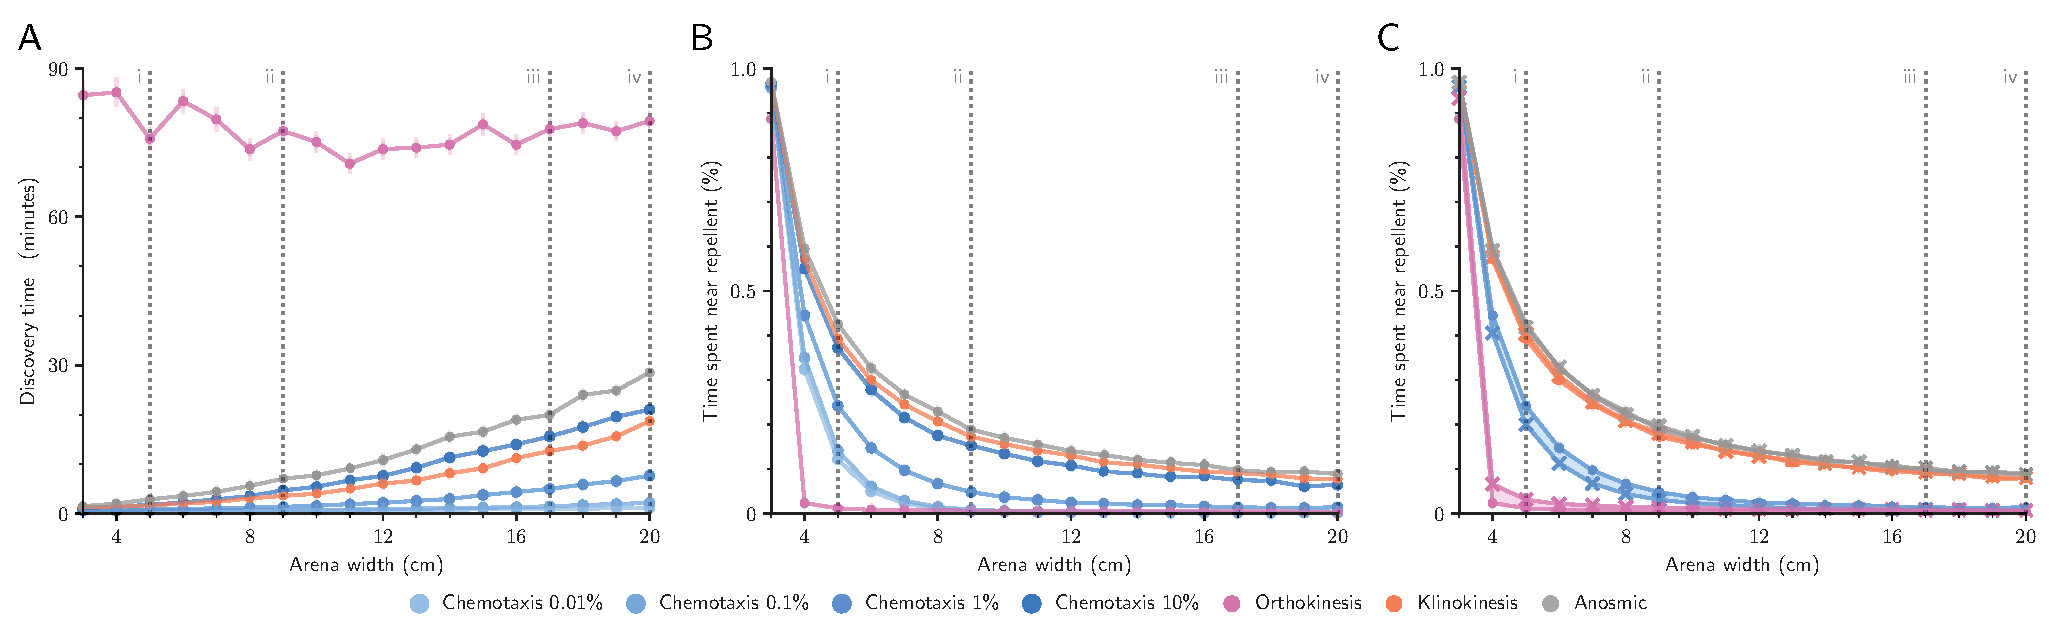
\includegraphics[width=\linewidth]{Figures/images/S4.eps}
  \caption{\textbf{ Simulation results are not affected by chemotactic sensitivity, or by substituting the starved and fed empirical datasets in the repellent-avoidance task.} A: Time elapsed before simulated larvae discovered food in the foraging task (mean ${\pm}$ standard error). Chemotaxis ${\%}$ values indicate the lowest concentration difference detectable by simulated larvae during each time step (2fps). B: Time spent in high-repellent areas during the repellent-avoidance task (mean ${\pm}$ standard error). All chemotactic sensitivities performed worse than the chemokinesis model. C: Starved simulations (X markers) and fed simulations (dots) performed similarly well during the repellent-avoidance task (mean ${\pm}$ standard error, shaded regions show difference between fed and starved simulations). In all panels, dashed grey lines correspond to ecologically relevant habitat sizes described in Table 2.}
\end{figure}